% !TEX root = ../report.tex
\chapter{Bestehende Arbeiten}
\begin{Spacing}{\mylinespace}
\begin{figure}[h!]
	\centering
	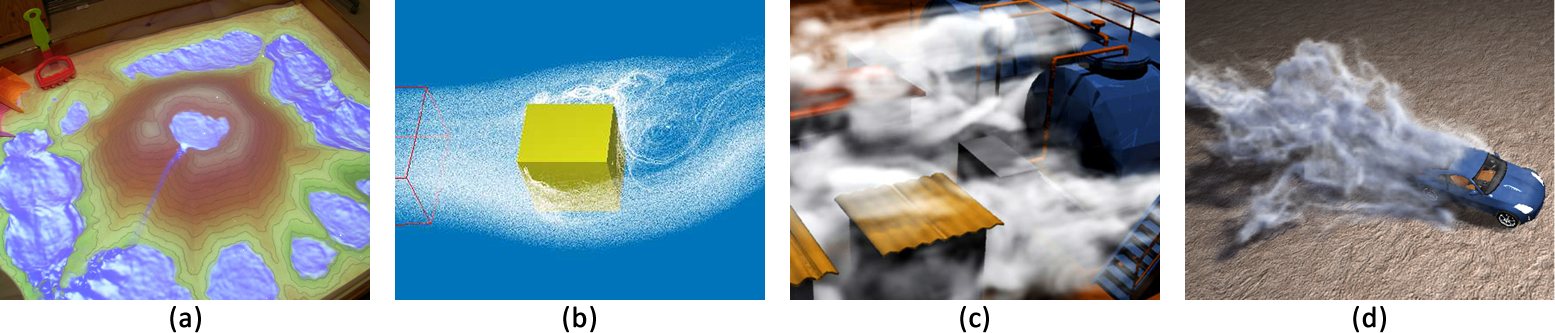
\includegraphics[width=\textwidth]{graphics/relatedWork.png}
	\caption{(a) Augmented Reality Sandbox. (b) A Particle System
for Interactive Visualization of 3D Flows. (c) Synthetic Turbulence using Artificial Boundary Layers. (d) Scalable Fluid Simulation using Anisotropic Turbulence Particles}
	\label{fig:relatedWork}
\end{figure}
Bevor wir auf unsere eigene Arbeit eingehen, wollen wir kurz einige andere Arbeiten vorstellen die sich mit ähnlichen Themen beschäftigen und an denen wir uns zum Teil orientiert haben.
\\\\
Beginnen wollen wir mit der \textit{Augmented Reality Sandbox} \cite{Kreylos2010} einem beeindruckenden Projekt der \textit{University of California} in Zusammenarbeit mit weiteren Forschungsinstituten, welches die Grundidee zu unserer Integrierung der Kinect 3D Kamera von Microsoft und dem Sandkasten lieferte. Ziel dieses Projekts war es, mit Hilfe der Kinect Kamera, eine spielerische Möglichkeit zu entwickeln, die es erlaubt topologische Landschaft, durch formen des Sandes mit den eigenen Händen, zu erstellen. Zusätzlich nutzen sie auch ein physikalisches System zur Simulation von Wasser die man in Abbildung \ref{fig:relatedWork} gut erkennen kann.
\\\\
Mit physikalischen System in Bezug auf Strömungssimulation beschäftigen sich auch die folgenden Arbeiten. \textit{A Particle System
for Interactive Visualization of 3D Flows} \cite{Krueger2005} ist zwar schon etwas älter, aber es ist eine der ersten Arbeiten in der mit der Auslagerung der Physikberechnung auf die GPU, um realistische Echtzeitströmungen zu simulieren, experimentiert wird. Zudem werden sehr interessante Konzepte nutzt, wie zum Beispiel die Speicherung der Partikelpositionen in einer Textur die gleichzeitig als Ein- und Ausgabecontainer zwischen den einzelnen Berechnungsschritten dient.
\\\\
Eine weitere interessante Arbeit ist \textit{Synthetic Turbulence using Artificial Boundary Layers} \cite{Pfaff2009}. Hier werden vorberechnete Strömungsfelder zur Simulation der Partikel genutzt umso extrem realistische Darstellungen zu realisieren. Durch die Vorberechnung verfügt dieses Verfahren aber leider über keine Echtzeitfähigkeit. In der Folgearbeit \textit{Scalable Fluid Simulation using Anisotropic Turbulence Particles} \cite{Pfaff2010} wird dieses Manko, durch starke Parallelisierung und der Berechnung vieler kleineren Einzelsimulationen, allerdings behoben.



\end{Spacing}
\newpage
\clearpage
%% End Of Doc